\paragraph{Солнечные столбы}

\begin{wrapfigure}[10]{r}{0.3\tw} 
    \vspace{-1pc}
    \centering
    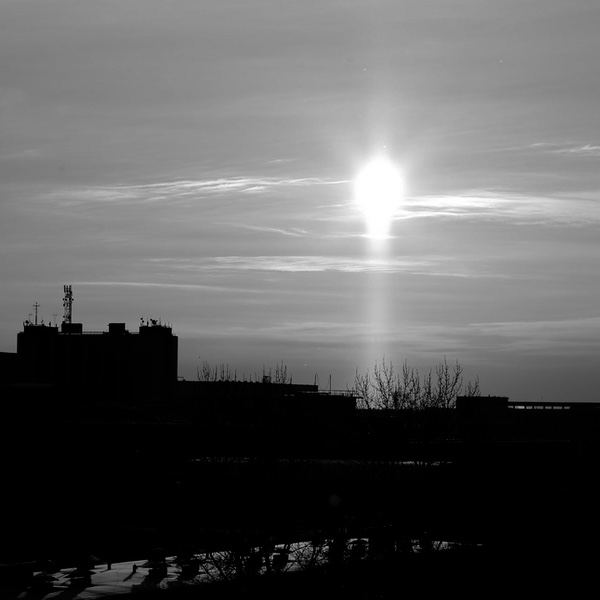
\includegraphics[width = 0.3\tw]{pillars}
    \caption{Солнечные столбы на восходе}
    \label{pic:pillars}
\end{wrapfigure}
Это узкие столбы света, которые визуально исходят от Солнца вертикально вверх, а иногда и вниз. Их высота может достигать 5\,--\,$10^\circ$, а иногда и больше. Солнечные столбы не являются вертикальными лучами, на самом деле они представляют собой отражение Солнца в миллионах кристаллов льда. Иногда они выглядят как несколько вертикально расположенных световых пятен, в зависимости от расположения облачных кристаллов.

Солнечные столбы формируются пластинчатыми кристаллами, которые, дрейфуя в окологоризонтальном положении, отражают солнечный свет в вертикальной плоскости. Высота столбов определяется зависимостью коэффициента отражения от угла падения света на основания ледяных кристаллов и высотой Солнца над горизонтом, суть углом падения света на отражающую поверхность.


